\section{Throughput for Writes (90 pts)}

\subsection{Full System}

In this section, we investigate the write-only workload performance characteristics of the full system, with the setup listed below. Figure~\ref{fig:4.1performance} is the response time and throughput measured by the middlewares with regard to the number of clients. The throughput and response time measured by memtier (not shown) is verified to follow the interactive law. Similar to the case in Section 3.2, the pressure on the network thread is relieved by doubling the middleware, so that it does not become the bottleneck, and we can confirm this by solely introducing the network RTT as think time, which turns out it indeed fits the interactive law at the middleware.

% Connect three load generating VMs to two middlewares and three memchached servers. Run a write-only experiment. 
% You need to plot throughput and response time measured on the middleware as a function of number of clients. The measurements have to be performed for 8, 16, 32 and 64 worker threads inside each middleware.

\begin{center}
	\scriptsize{
		\begin{tabular}{|l|c|}
			\hline Number of servers                & 3          \\ 
			\hline Number of client machines        & 3          \\ 
			\hline Instances of memtier per machine & 2          \\ 
			\hline Threads per memtier instance     & 1          \\
			\hline Virtual clients per thread       & [1, 2, 4, 6, 8, 16, 24, 32, 36, 40, 44]    \\ 
			\hline Workload                         & Write-only \\
			\hline Multi-Get behavior               & N/A        \\
			\hline Multi-Get size                   & N/A        \\
			\hline Number of middlewares            & 2          \\
			\hline Worker threads per middleware    & [8, 16, 32, 64]    \\
			\hline Repetitions                      & 3 $\times$ 80 seconds each  \\ 
			\hline 
		\end{tabular}
	} 
\end{center}

\begin{figure}[!h]
\parbox{.5\linewidth}{
\centering
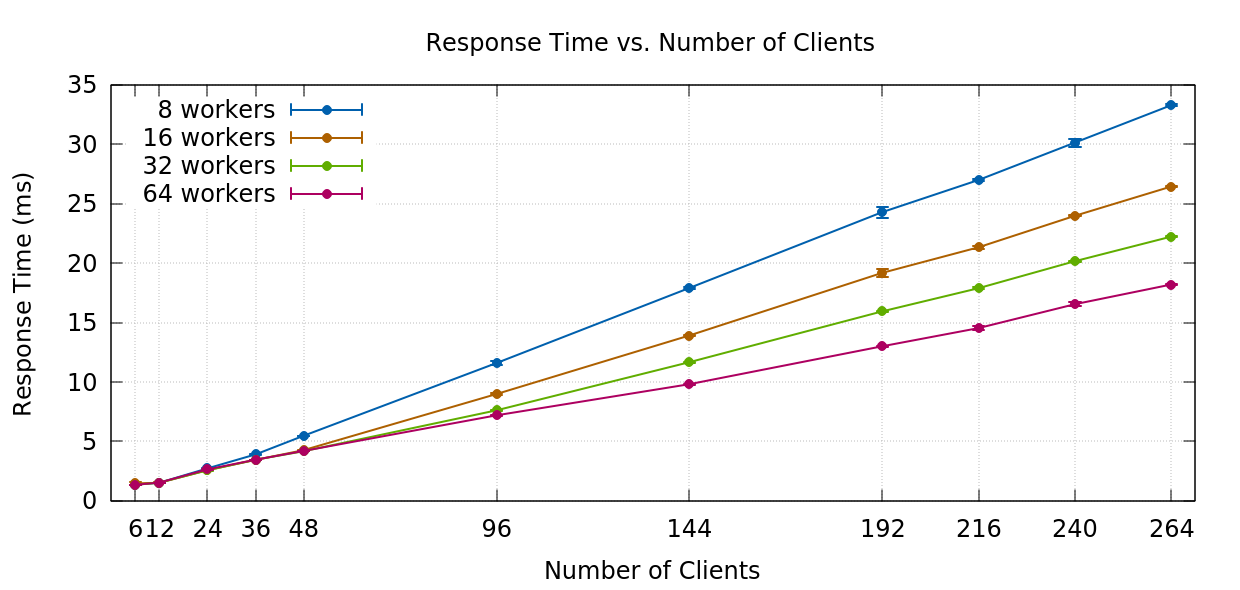
\includegraphics[width=0.5\textwidth]{img/4_responsetime_mw.png}
}
\parbox{.5\linewidth}{
\centering
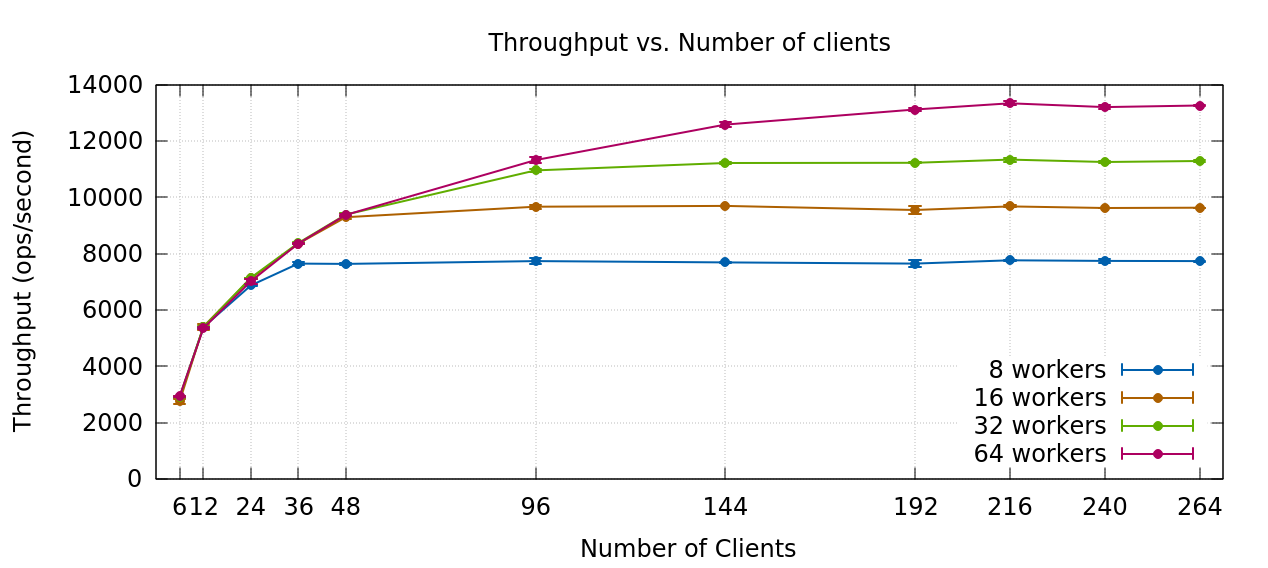
\includegraphics[width=0.5\textwidth]{img/4_throughput_mw.png}
}
\captionsetup{justification=centering}
\caption{\label{fig:4.1performance}Full System Write-only Performance Measured on Two Middlewares \\(Error bars are too small to be distinguished)}
\end{figure}

\subsubsection{Explanation}

% Provide a detailed analysis of the results (e.g., bottleneck analysis, component utilizations, average queue lengths, system saturation). Add any additional figures and experiments that help you illustrate your point and support your claims.
The difference between this section and Section 3.2 is that the number of servers is increased to three. For write-only workload, we expect a throughput decrease introduced by this, because the middlewares will have to replicate the \texttt{SET} operation to every server, resulting in a increase in the time spent communicating with servers (the service time). The experiment results indeed match our prediction: the maximum throughputs (listed in the table of Section 4.2), which are hit at 36, 48, 96, 192 clients respectively for 8, 16, 32, 64 workers, are always lower than the maximum throughput with the same number of workers in Section 3.2; and the service times are always higher than those of Section 3.2, as shown by the all-positive values in Figure~\ref{fig:4.1servicediff}. To make it clear, the saturation points are chosen in such a way that further increasing clients will never introduce a throughput gain larger than 5\%, while the response time will grow almost linearly. The steep scaling of average queue length when going beyond the chosen saturation points, as plotted in Figure~\ref{fig:4.1queue}, also supports our choice.


\begin{figure}[!h]
\parbox{.5\linewidth}{
\centering
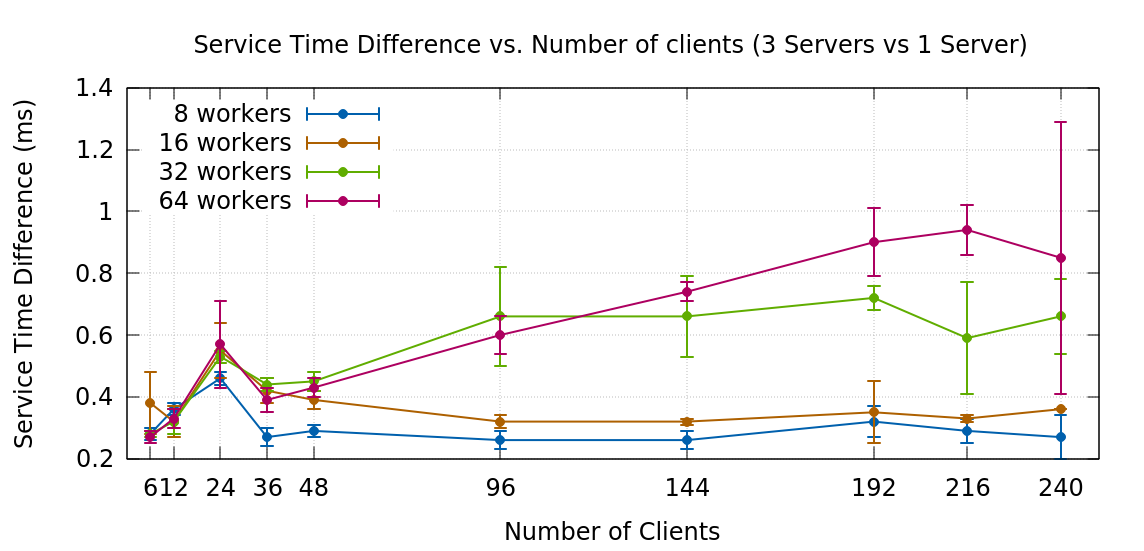
\includegraphics[width=0.5\textwidth]{img/4_servicediff.png}
\captionsetup{justification=centering}
\caption{\label{fig:4.1servicediff}Service Time Differences\\Between Sections 4 and 3.2}
}
\parbox{.5\linewidth}{
\centering
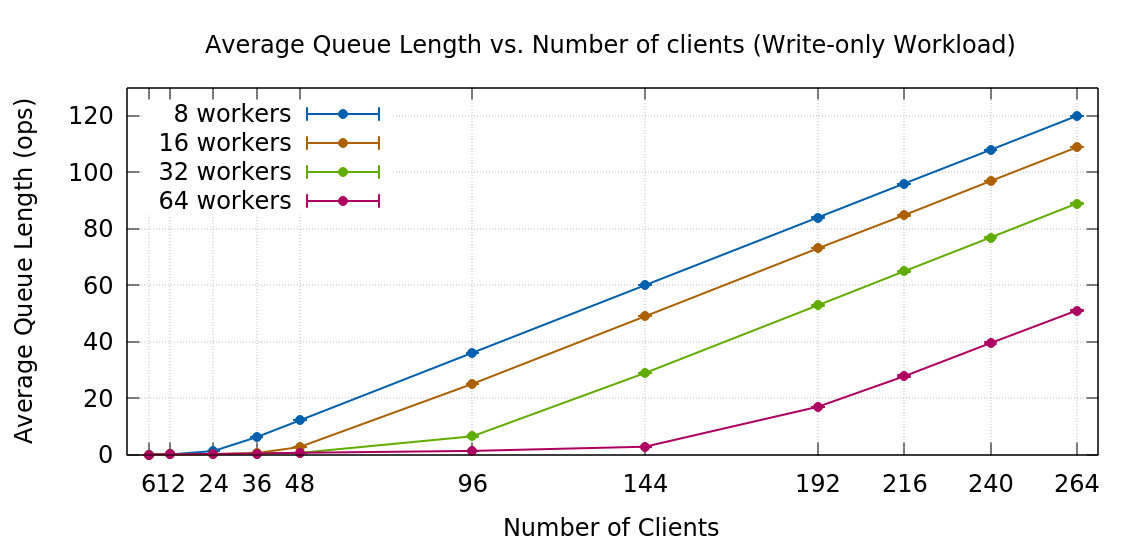
\includegraphics[width=0.5\textwidth]{img/4_queuelen.png}
\captionsetup{justification=centering}
\caption{\label{fig:4.1queue}Average Queue Length\\(Error bars are too small to be distinguished)}
}
\end{figure}

As the maximum throughput in this section never reaches the maximum write-only throughput that a server can handle (which was measured to be about 15000 ops/sec by Section 2.1 One Server baselines), the bottleneck is again not in the server side, but in the middleware itself. This can be proved by the time breakdown as in Figure~\ref{fig:4.1breakdown}: when there are only 8 workers, most time is spent in waiting in the request queue; as the number of worker threads increases, the waiting time decreases because more requests can be processed in parallel, and the memcached service time increases because more load is put on the servers, resulting in longer processing time. If the bottleneck was the memcached servers, when the number of worker threads is fixed and the number of clients increases, the service time should also be increased due to server saturation, but it is not the case, because the bottleneck is the number of worker threads of the middlewares, which determines how many clients (requests) the memcached servers should deal with. We also find that the response time discrepancy between middleware and memtier measurements is equal to the network RTT, indicating that the waiting time in the OS network queue is about zero, thus the network thread does not become a bottleneck.

\begin{figure}[!h]
\centering
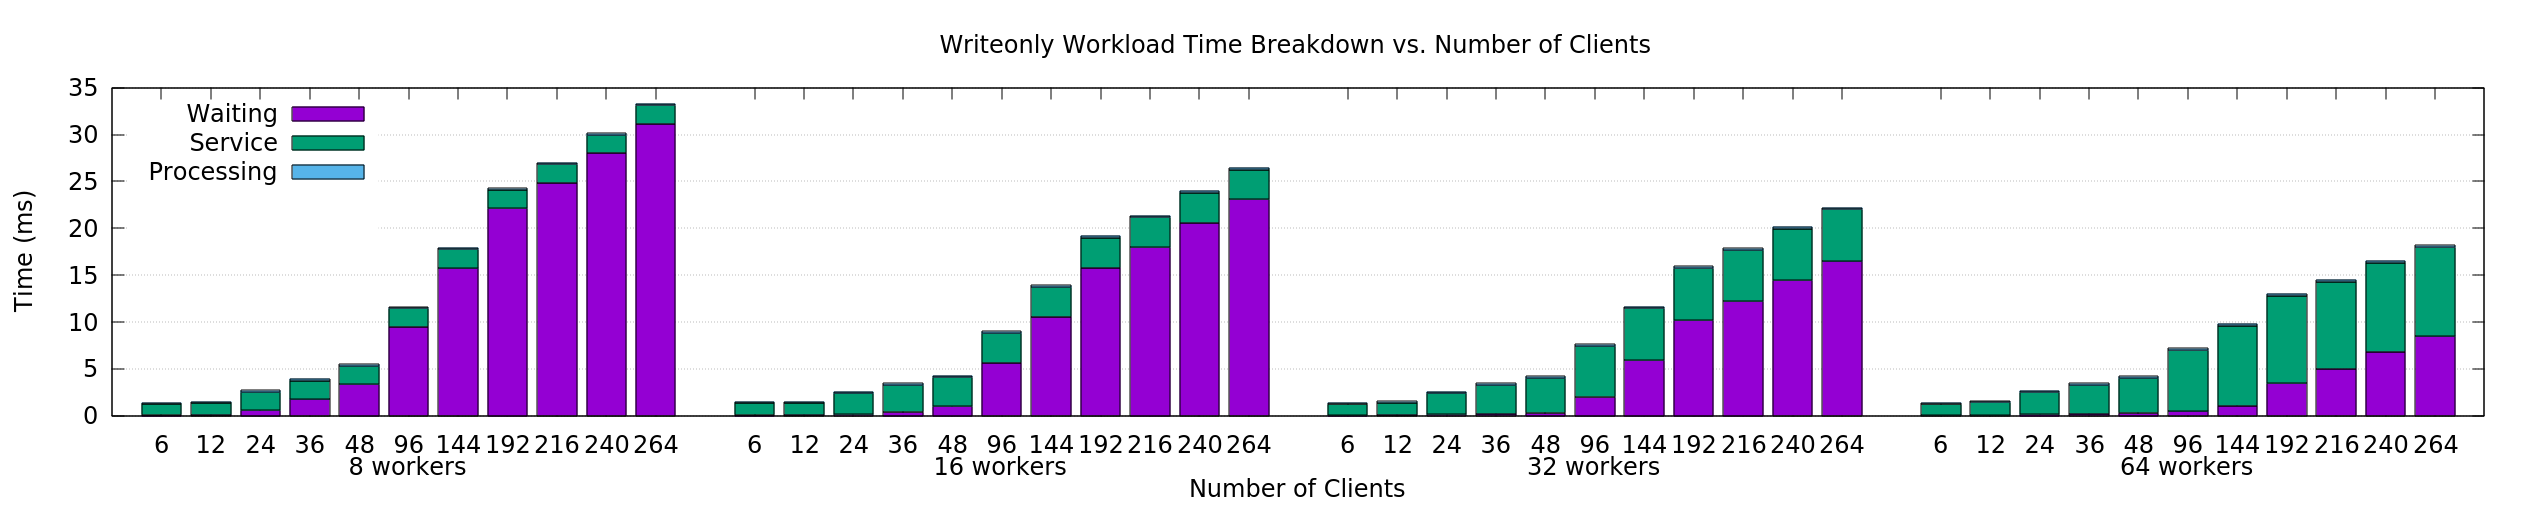
\includegraphics[width=1.0\textwidth]{img/4_breakdown.png}
\captionsetup{justification=centering}
\caption{\label{fig:4.1breakdown}Middleware Time Breakdown in Two Middlewares (Write-only Workload) \\(Errors are too small to be seen)}
\end{figure}

\subsection{Summary}

% Based on the experiments above, fill out the following table with the data corresponding to the maximum throughput point for all four worker-thread scenarios.

% 36(6) 48(8) 96(16) 192(32)
\begin{center}
	{Maximum throughput for the full system}
	\begin{tabular}{|l|p{1.5cm}|p{1.5cm}|p{1.5cm}|p{1.5cm}|}
		\hline                                            & WT=8 & WT=16 & WT=32 & WT=64 \\ 
		\hline Throughput (Middleware)                    & 7645.00     &   9291.08    &  10954.73     & 13117.29      \\ 
		\hline Throughput (Derived from MW response time) & 7501.04     &	9275.36     &	11198.45    &	13587.20     \\ 
	    \hline Throughput (Client)                        & 7562.64     &   9214.13    &  10842.41     & 12932.08      \\ 
		\hline Average time in queue                      &  1.79   &  1.02     &   1.97    &   3.45    \\ 
		\hline Average length of queue                    &  6.21   &  2.71     &   6.51    &   16.95    \\ 
		\hline Average time waiting for memcached         &  1.97   &  3.08     &   5.46    &   9.32    \\ 
		\hline 
	\end{tabular}
\end{center}

To derive throughput from MW response time correctly with the interactive law, the mean \texttt{ping} latency is considered as the think time. Note that our gathered \texttt{ping} logs show that network latencies are relatively unstable, and the standard deviations in each single repetition are often 50\%$\sim$100\% of the average latency, so using the average RTT as the think time is just a best-effort estimation, which can explain why the derived throughputs, while fitting the measured values fairly well, do have an error of less than 5\% from the direct measurements.

For the 64 worker threads case, the average waiting time, service time and queue length is noticeably higher than the other cases, this should be because at this state the system is already saturated, and even an adequately smaller number of clients between 144 and 192 is also able to saturate the system, but our testing points are limited and did not include that precise number of clients. Increasing from that number to our chosen number of clients (192) have resulted in the increase of the aforementioned metrics. Similar argument holds for the 32 workers case, only that it is not as severe as 64 workers.

From the table and the data from previous experiments, we can see that the maximum throughput in each column is about 2000 ops/sec less than the maximum throughput in Section 3.2 with the same number of worker threads. Also, by comparing the average time waiting for memcached with Section 3.2 (i.e. the service time difference as compared in Figure~\ref{fig:4.1servicediff}), it shows that adding more servers indeed introduces more overhead in the service time, thus lowering the throughput the system can reach. Further, we observe that the service time also has a positive correlation with the number of worker threads, because with more workers the middleware is able to push more load to the servers, and the servers will yield higher service time under heavier load.

By looking at the average length of queue and the average time in queue, we find that when the system reaches the maximum throughput, the averge queue length will be much larger than in a under-saturated state, because more requests will have to wait longer in the queue, as all workers are busy. On the other hand, Figure~\ref{fig:4.1queue} shows that for the same number of clients, the more worker threads we have, the lower average queue length we get, despite that the throughput also increases. This is because with more workers, more requests will be under processing by the workers, instead of being waiting in the queue. With more workers, it will be more difficult to make the average queue length grow explosively when adding more clients.
